% =====================================================================
% Snippet: metrics-card.tex
% =====================================================================
% USAGE: A single metric card showing a key number ("FID = 3.17") with
% optional comparison vs baseline. Examples 08 Diffusion uses this
% pattern ("FID = 3.17 on CIFAR-10") at the figure bottom.
%
% Two variants:
%   A. Single metric (big number + label)
%   B. With baseline comparison (delta + arrow up/down)
%
% Copy whichever fits.
% =====================================================================

\documentclass[tikz,border=10pt]{standalone}
\usepackage{xcolor,tikz}
\usetikzlibrary{positioning,calc}

\definecolor{acaBlueLine}{HTML}{3060A8}
\definecolor{acaBlueFill}{HTML}{DCE6F4}
\definecolor{acaGreenLine}{HTML}{389050}
\definecolor{acaGreenFill}{HTML}{DBEDDC}
\definecolor{acaOrangeLine}{HTML}{D06020}
\definecolor{acaGreyLine}{HTML}{606060}

\begin{document}
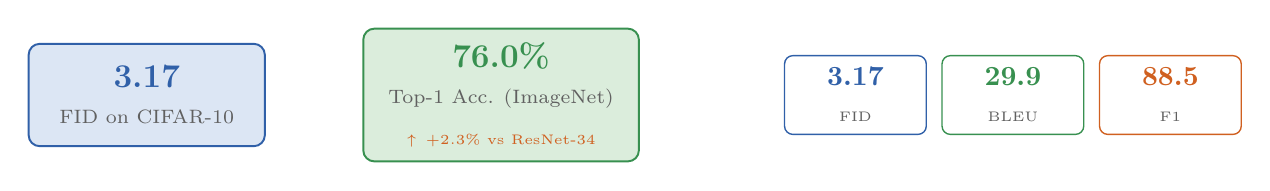
\begin{tikzpicture}

%% COPY-START (Variant A — Single metric, FID-style) =================
% Note: use \large (not \Large) — figure-embedded cards should match
% surrounding box font weight. \Large breaks visual hierarchy.
\node[draw=acaBlueLine, fill=acaBlueFill, rounded corners=4pt,
      line width=0.7pt, minimum width=3.0cm, minimum height=1.3cm,
      align=center, inner sep=5pt]
  (cardA) at (0, 0) {%
    {\large\bfseries\color{acaBlueLine} 3.17}\\[1pt]
    {\scriptsize\color{acaGreyLine} FID on CIFAR-10}
  };
%% COPY-END Variant A ================================================


%% COPY-START (Variant B — With baseline comparison) =================
\node[draw=acaGreenLine, fill=acaGreenFill, rounded corners=4pt,
      line width=0.7pt, minimum width=3.5cm, minimum height=1.5cm,
      align=center, inner sep=5pt]
  (cardB) at (4.5, 0) {%
    {\large\bfseries\color{acaGreenLine} 76.0\%}\\[1pt]
    {\scriptsize\color{acaGreyLine} Top-1 Acc. (ImageNet)}\\[3pt]
    {\tiny\color{acaOrangeLine}$\uparrow\,+2.3\%$ vs ResNet-34}%
  };
%% COPY-END Variant B ================================================


%% COPY-START (Variant C — Multi-metric strip) =======================
\foreach [count=\i] \val/\lab/\col in {%
  3.17/FID/acaBlueLine,%
  29.9/BLEU/acaGreenLine,%
  88.5/F1/acaOrangeLine%
} {
  \pgfmathsetmacro\cx{9 + (\i - 1) * 2.0}
  \node[draw=\col, fill=white, rounded corners=3pt,
        line width=0.5pt, minimum width=1.8cm, minimum height=1.0cm,
        align=center, inner sep=3pt]
    at (\cx, 0) {%
      {\normalsize\bfseries\color{\col} \val}\\[1pt]
      {\tiny\color{acaGreyLine} \lab}%
    };
}
%% COPY-END Variant C ================================================

\end{tikzpicture}
\end{document}
